\chapter{Snippets}

{\setlength{\parindent}{0cm}
    \section*{Common Elements}
    \textasciitilde~$\sim$ \# \$ \% \^{} \& \_ \{ \} \~{} \textbackslash{} \~a \^a
    \hfill
    normal text {\itshape walzing \bfseries Wombat} more normal text%
    \footnote{An example footnote.}
    
    $ \hat{o} \widehat{oo} \tilde{o} \dot{o} \bar{o} \vec{o} \hat{\imath} \vec{\jmath} $
    $ a' a'' \not{a} \overrightarrow{AB} \overline{a} \underline{a} $

    % \emph is a command with argument, \em is a switch
    \emph{emphasized text}, this part is normal
    \hfill
    {\em emphasized text}, this part is normal
    
    Mr.~Nonbreaking~Space\textsubscript{sub}\textsuperscript{sup}
    \hfill
    \today
    
    `quote'~-- ``quote''~--- \hfill $3-2=1$ \hfill \verb;\textbf{Hi mate!};\ldots
    
    \begin{itemize}
        \item item
        \item another item
    \end{itemize}

    \begin{enumerate}
        \item the first item
        \begin{enumerate}
            \item item 1.a
            \item item 1.b
        \end{enumerate}
    \item the second item
    \end{enumerate}

    \begin{tabular}{r|*{2}{|c}|l}
        \# & \multicolumn{3}{c}{Columns}\\
        \hline
        111 & 222 & 222 & 333\\
        \hline
        4 & \multirow{2}{*}{58} & 5 & 6\\
        \cline{1-1}
        7 & & 8 & 9\\
    \end{tabular}

    \begin{table}
        \begin{center}
            \begin{tabular}{|lcr|}
                \hline
                1 & 2 & 3\\
                4 & 5 & 6\\
                7 & 8 & 9\\
                \hline
            \end{tabular}
            \caption[]{A simple table.}
        \end{center}
    \end{table}

    Label/ref prefixes:
    ch:x (chapter), sec:x (section), subsec:x (subsection),
    fig:x (figure), tab:x (table), eq: (equation),
    thm:x (theorem), lem:x (lemma), def:x (definition), pro:x (proposition),
    lst:x (code listing), itm:x (enumerated list item),
    alg:x (algorithm), app:x (appendix subsection)
    
    \begin{equation}
        \label{eq:snippet}
        x^2 - 5 x + 6 = 0
    \end{equation}
    
    See equation~\ref{eq:snippet} for more details.
    Alternatively, see \eqref{eq:snippet}, or go to \autoref{app:meetings},
    or just use \autoref{alg:snippet-euclid} from line~\ref{alg:snippet-euclidendwhile}.

    % The link location will be placed on the line below
    %\phantomsection
    %\label{the_label}
    
    \begin{figure}
        \centering
        \subfloat[label 1]{{
            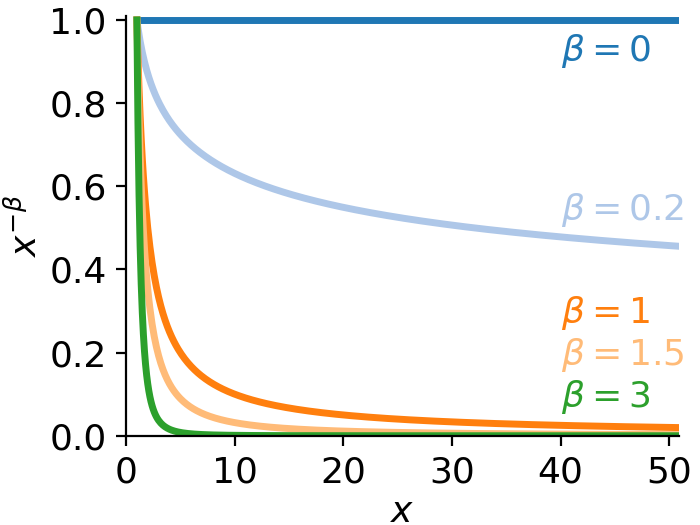
\includegraphics[scale=0.75]{images/generated/power-law}
            \label{fig:snippet-power-law-a}
        }}
        \qquad
        \subfloat[label 2]{{
            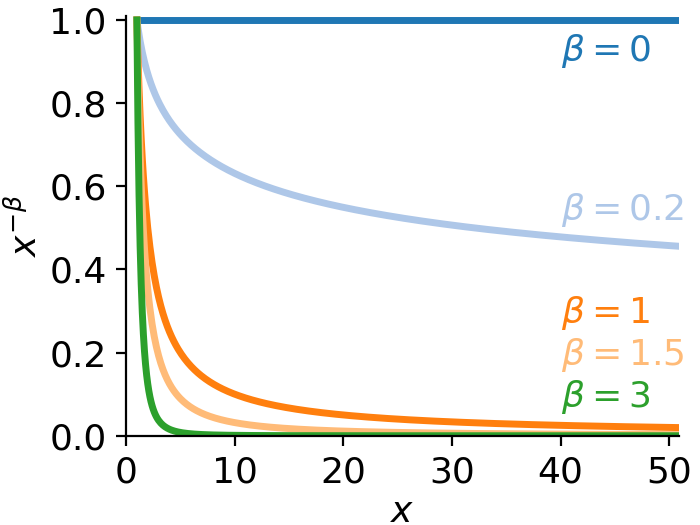
\includegraphics[scale=0.75]{images/generated/power-law}
        }}
        \caption[]{Two figures side by side.}
        \label{fig:snippet-power-law}
    \end{figure}
    
    More references: \autoref{fig:snippet-power-law} \& \autoref{fig:snippet-power-law-a}.

    \section*{Technical Texts}

    \subsection*{Mathematics}
    
    Inline math is $(ea+sy)^n$. Displayed equation:
    \[
    3\times7\text{ apples}=21\textit{ bananas}
    \qquad\qquad
    % (,=3 :=4 ;=5 !=-3)/18 of quad
    s\,p\:a\;c\quad i\qquad ng n\!g
    \]
    
    $\alpha\beta\Rightarrow\bm{\alpha\beta}$
    $\implies 1\overset{(note)}{\leq}2$

    Small $\sum_{i=0}^n x_i$ vs
    $\displaystyle \lim_{x \to \infty}\sum_{i=0}^{n}x_i=0 \qquad$
    $\displaystyle\prod_{\substack{i\ge0\\j\le0}}x_i=0 \qquad$
    $f(x)|_{x_1=0}=1 \qquad$
    $\binom{n}{k}=\frac{n!}{k!(n-k)!}$
    
    $\frac{x}{y}$ vs $\tfrac{x}{y}$ vs $\dfrac{x}{y}$ vs $^x/_y \qquad$
    $\sqrt[n]{1+x+\dots+x^n}\qquad$
    $(a),[b],\{c\},|d|,\|e\|,\langle f \rangle,$
    $\lfloor g \rfloor,\lceil h \rceil,\ulcorner i \urcorner$
    
    $5 \bmod 2=1 \qquad 5 \equiv 1 \mod 2 \qquad 5 \equiv 1 \pmod 2 \qquad$
    $\{\frac{x}{y}\}$ vs $\left\{\frac{x}{y}\right\}$
    
    $A=\left(x\;\middle|\;x\in[-1,1]\backslash\{0\} \land x\neq\pm2\right)$
    $\qquad \mathbb{N}\mathbb{Z}\mathbb{Q}\mathbb{R}\mathbb{C}$
    
    \[A=
    \begin{pmatrix}
        a & \cdots & b\\
        \vdots & \ddots & \vdots\\
        c & \cdots & d
    \end{pmatrix}
    \qquad B=
    \begin{array}{c|c}
        1 & 2\\
        \hline
        3 & 4
    \end{array}
    \qquad f(n)=
    \begin{cases}
        n/2       & \quad \text{if } n \text{ is even}\\
        -(n+1)/2  & \quad \text{if } n \text{ is odd}
    \end{cases}
    \]
    
    \subsection*{Advanced Mathematics}
    
    %todo equation [w/ split inside], multline, gather, align
    \ldots
    
    \begin{algorithm}
        \caption{Euclid's algorithm}
        \label{alg:snippet-euclid}
        \begin{algorithmic}
            \Procedure{Euclid}{$a,b$}\Comment{The g.c.d. of a and b}
            \State $r\gets a\bmod b$
            \While{$r\not=0$}\Comment{We have the answer if r is 0}
            \State $a\gets b$
            \State $b\gets r$
            \State $r\gets a\bmod b$
            \EndWhile\label{alg:snippet-euclidendwhile}
            \State \textbf{return} $b$\Comment{The gcd is b}
            \EndProcedure
        \end{algorithmic}
    \end{algorithm}

    This is $\overset{top}{something}$.
    
    \subsection*{Theorems}
    
    \begin{theorem}[Pythagorean theorem]
        \label{thm:snippet-pythagorean}
        Content.
    \end{theorem}
    
    \begin{corollary}
        Content.
    \end{corollary}
    
    \begin{corollary}
        Content.
    \end{corollary}
    
    \begin{lemma}
        \label{lem:snippet-lemma1}
        Content.
    \end{lemma}
    
    \begin{proof}
        Trivial.
    \end{proof}
    
    \begin{proof}[Proof of~\autoref{thm:snippet-pythagorean}]
        Use~\autoref{lem:snippet-lemma1}.
    \end{proof}

    \begin{definition}
        Something is \textit{something} if\ldots
    \end{definition}
}
